\documentclass[tikz, border=10pt]{standalone}

\usepackage{tikz}

\usepackage[T1]{fontenc}

\begin{document}
  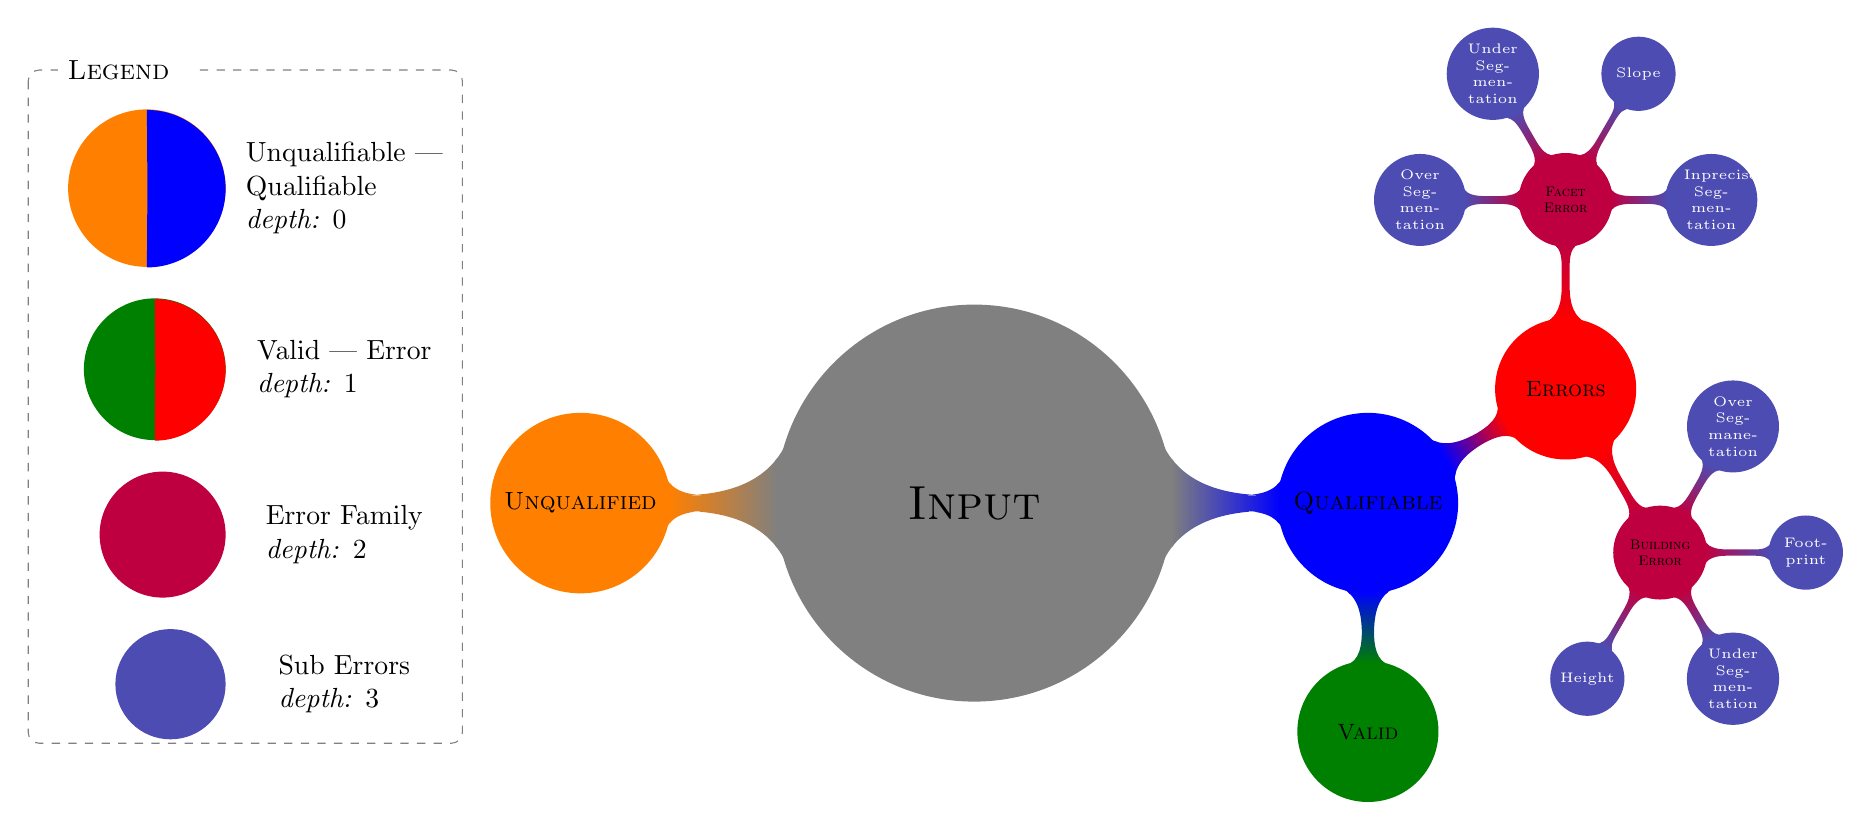
\begin{tikzpicture}
    \usetikzlibrary{mindmap, trees, decorations.pathreplacing}
    \path[mindmap, concept color=black!50, text=black]
      node (input) [concept, minimum size=5cm]{\LARGE\textsc{Input}}[clockwise from=0]
      child[concept color=orange, text=black, grow=180]
      {
        node[concept]{\textsc{Unqualified}}[clockwise from=180]
      }
      child[concept color=blue, text=black, grow=0]{
      	node[concept]{\textsc{Qualifiable}}
      	child[concept color=black!50!green, grow=270]{
      		node[concept]{\textsc{Valid}}
      	}
      	child[concept color=red, grow=30]{
      		node[concept]{\textsc{Errors}}
      		child[concept color=purple, text=black, grow=90]
      		{
      			node[concept]{\textsc{Facet Error}}
      			child[concept color=blue!70!yellow, text=white, grow=180]
      			{
      				node[concept]{Over Segmentation}
      			}
      			child[concept color=blue!70!yellow, text=white, grow=120]
      			{
      				node[concept]{Under Segmentation}
      			}
      			child[concept color=blue!70!yellow, text=white, grow=0]
      			{
      				node[concept]{Inprecise Segmentation}
      			}
      			child[concept color=blue!70!yellow, text=white, grow=60]
      			{
      				node[concept]{Slope}
      			}
      		}
      		child[concept color=purple, text=black, grow=300]
      		{
      			node[concept]{\textsc{Building Error}}
      			child[concept color=blue!70!yellow, text=white, grow=60]
      			{
      				node[concept]{Over Segmanetation}
      			}
      			child[concept color=blue!70!yellow, text=white, grow=300]
      			{
      				node[concept]{Under Segmentation}
      			}
      			child[concept color=blue!70!yellow, text=white, grow=0]
      			{
      				node[concept]{Foot-\\print}
      			}
      			child[concept color=blue!70!yellow, text=white, grow=240]
      			{
      				node[concept]{Height}
      			}
      		}
      	}
      };

      \path (input.west) + (-7, 4) node[circle, fill, color=orange, minimum size=2cm, anchor=east] (1) {};
      \fill[color=blue] (1.east) + (-1,0) -- (1.south) arc (-90:90:1) -- cycle;
      \path (1.east) + (1.5, 0) node[text=black, align=left] {Unqualifiable |\\Qualifiable\\\textit{depth:} $0$};

      \path (input.west) + (-7, 1.7) node[circle, fill, color=black!50!green, minimum size=1.8cm, anchor=east] (2) {};
      \fill[color=red] (2.east) + (-.9,0) -- (2.south) arc (-90:90:.9) -- cycle;
      \path (2.east) + (1.5, 0) node[text=black, align=left] {Valid | Error\\\textit{depth:} $1$};

      \path (input.west) + (-7, -.4) node[circle, fill, color=purple, minimum size=1.6cm, anchor=east] (3) {};
      \path (3.east) + (1.5, 0) node[text=black, align=left] {Error Family\\\textit{depth: }$2$};

      \path (input.west) + (-7, -2.3) node[circle, fill, color=blue!70!yellow, minimum size=1.4cm, anchor=east] (4) {};
      \path (4.east) + (1.5, 0) node[text=black, align=left] {Sub Errors\\\textit{depth:} $3$};

      \path (4.east) + (3, -.75) node (8) {};
      \path[rounded corners, draw=black!50, dashed] (1.west) + (-.5, 1.5) rectangle (8);
      \path (1.west) + (.75, 1.5) node[fill=white, text width= 1.5cm] (legend) {\textsc{Legend}};

  \end{tikzpicture}
\end{document}
